\documentclass[12pt]{book}
\usepackage{fontspec}
\setmainfont{TeX Gyre Pagella}
\usepackage[paperwidth=8in,paperheight=8in,margin=0.6in]{geometry}
\usepackage{xcolor}
\usepackage{amssymb}
\usepackage{tikz}
\usetikzlibrary{arrows.meta}
\pagestyle{empty}
\setlength{\parindent}{0pt}

\newcommand{\artnote}[1]{{\color{gray!70}\small\itshape [Illustration: #1]}\par\vspace{0.3in}}
\newcommand{\bigline}[1]{{\Huge #1}\par}
\newcommand{\pagenum}[1]{\vfill{\color{gray!50}\footnotesize #1}}
\newcommand{\sprollpage}{\newpage\vspace*{0.4in}}

\begin{document}

\thispagestyle{empty}
\begin{center}
\vspace*{1.1in}
{\Huge \textbf{SPROLL 08}}\\[0.4in]
{\huge \textbf{When Are They Equal?}}\\[0.5in]
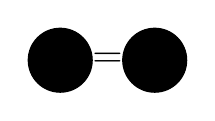
\begin{tikzpicture}
\filldraw[fill=black] (-0.7,0) circle (0.16in);
\filldraw[fill=black] (0.5,0) circle (0.16in);
\node at (-0.1,0) {\Large =};
\end{tikzpicture}
\\[0.4in]
{\large \textit{a question you check, not one you guess}}\\[0.3in]
{\small The Sproll Curriculum $\cdot$ Cycle I: Pops}
\end{center}

\sprollpage
\begin{center}
\vspace*{1.5in}
{\Large The Sproll Curriculum}\\[0.2in]
{\normalsize Cycle I --- Pops: Things, Differences, and Counting}\\[0.6in]
{\small Sproll 08 of 40 \quad $\cdot$ \quad follows Sproll 07: Same Picture, Different Story}
\end{center}
\pagenum{2}

\sprollpage
\begin{center}
\vspace*{0.5in}
\artnote{two empty piles or boxes, unlabeled, from the end of Sproll 07}

\begin{tikzpicture}
\draw[line width=1.5pt] (-1.5,-0.4) rectangle (-0.7,0.3);
\draw[line width=1.5pt] (0.7,-0.4) rectangle (1.5,0.3);
\end{tikzpicture}
\vspace{0.35in}
\bigline{Some rules sort everything}\vspace{0.1in}
{\Large into two piles: same, or not.}
\end{center}
\pagenum{3}

\sprollpage
\begin{center}
\vspace*{0.4in}
\artnote{four shapes waiting to be sorted: a black dot, a black square, an orange triangle, an orange circle}

\begin{tikzpicture}
\filldraw[fill=black] (-1.8,0) circle (0.13in);
\draw[line width=2pt] (-1.0,-0.13) rectangle (-0.6,0.13);
\draw[fill=orange!60] (0.3,-0.16) -- (0.5,0.16) -- (0.7,-0.16) -- cycle;
\draw[fill=orange!60] (1.5,0) circle (0.13in);
\end{tikzpicture}
\vspace{0.3in}
\bigline{Rule: same color.}
\end{center}
\pagenum{4}

\sprollpage
\begin{center}
\vspace*{0.4in}
\artnote{the same four shapes, now sorted into two labeled piles: black things in one pile, orange things in the other}
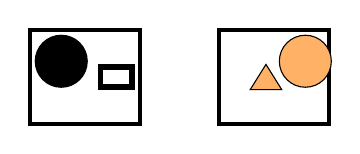
\begin{tikzpicture}
\draw[line width=1.5pt] (-1.9,-0.6) rectangle (-0.5,0.6);
\filldraw[fill=black] (-1.5,0.2) circle (0.13in);
\draw[line width=2pt] (-1.0,-0.13) rectangle (-0.6,0.13);
\draw[line width=1.5pt] (0.5,-0.6) rectangle (1.9,0.6);
\draw[fill=orange!60] (0.9,-0.16) -- (1.1,0.16) -- (1.3,-0.16) -- cycle;
\draw[fill=orange!60] (1.6,0.2) circle (0.13in);
\end{tikzpicture}
\vspace{0.3in}
\bigline{Two piles. Sorted by the rule.}
\end{center}
\pagenum{5}

\sprollpage
\begin{center}
\vspace*{0.8in}
\artnote{the black dot and black square, isolated together, with an equals sign between them}
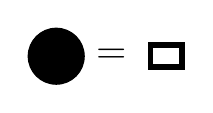
\begin{tikzpicture}
\filldraw[fill=black] (-0.7,0) circle (0.14in);
\node at (0,0) {\Large =};
\draw[line width=2pt] (0.5,-0.14) rectangle (0.9,0.14);
\end{tikzpicture}
\vspace{0.35in}
\bigline{Equal under this rule.}\vspace{0.1in}
{\Large Not because they look alike overall.}
\end{center}
\pagenum{6}

\sprollpage
\begin{center}
\vspace*{0.8in}
\artnote{the black dot and the orange circle, isolated together, with a not-equal mark between them despite being the same shape}
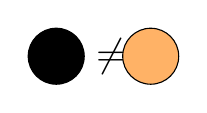
\begin{tikzpicture}
\filldraw[fill=black] (-0.7,0) circle (0.14in);
\node at (0,0) {\Large $\neq$};
\draw[fill=orange!60] (0.5,0) circle (0.14in);
\end{tikzpicture}
\vspace{0.35in}
\bigline{Not equal under this rule.}\vspace{0.1in}
{\Large Even though both are round.}
\end{center}
\pagenum{7}

\sprollpage
\begin{center}
\vspace*{0.7in}
\artnote{the same four shapes, calm and unsorted, with a small question mark hovering}

\begin{tikzpicture}
\filldraw[fill=black] (-1.8,0) circle (0.13in);
\draw[line width=2pt] (-1.0,-0.13) rectangle (-0.6,0.13);
\draw[fill=orange!60] (0.3,-0.16) -- (0.5,0.16) -- (0.7,-0.16) -- cycle;
\draw[fill=orange!60] (1.5,0) circle (0.13in);
\end{tikzpicture}
\vspace{0.3in}
\bigline{Equal does not mean ``looks the same.''}\vspace{0.1in}
{\Large It means: same answer, under the stated rule.}
\end{center}
\pagenum{8}

\sprollpage
\begin{center}
\vspace*{0.4in}
\artnote{the same four shapes, now re-sorted under a new rule into two different piles: round things in one, pointy or square things in the other}
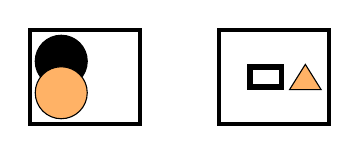
\begin{tikzpicture}
\draw[line width=1.5pt] (-1.9,-0.6) rectangle (-0.5,0.6);
\filldraw[fill=black] (-1.5,0.2) circle (0.13in);
\draw[fill=orange!60] (-1.5,-0.2) circle (0.13in);
\draw[line width=1.5pt] (0.5,-0.6) rectangle (1.9,0.6);
\draw[line width=2pt] (0.9,-0.13) rectangle (1.3,0.13);
\draw[fill=orange!60] (1.4,-0.16) -- (1.6,0.16) -- (1.8,-0.16) -- cycle;
\end{tikzpicture}
\vspace{0.3in}
\bigline{Rule: same shape, not color.}\vspace{0.1in}
{\Large Now the piles are different.}
\end{center}
\pagenum{9}

\sprollpage
\begin{center}
\vspace*{0.8in}
\artnote{the black dot and the orange circle, now shown equal under the new rule, with an equals sign between them}
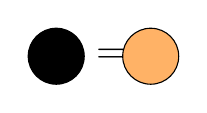
\begin{tikzpicture}
\filldraw[fill=black] (-0.7,0) circle (0.14in);
\node at (0,0) {\Large =};
\draw[fill=orange!60] (0.5,0) circle (0.14in);
\end{tikzpicture}
\vspace{0.35in}
\bigline{Change the rule, and equal can change too.}
\end{center}
\pagenum{10}

\sprollpage
\begin{center}
\vspace*{0.4in}
\artnote{the two full histories from Sproll 02 and 07, side by side, with a rule label and equals sign, then a second version with a different rule label and a not-equal sign}
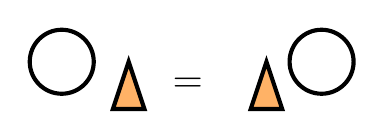
\begin{tikzpicture}
\draw[line width=1.5pt] (-2.2,0.3) circle (0.16in);
\draw[fill=orange!60, line width=1.5pt] (-1.55,-0.3) -- (-1.35,0.3) -- (-1.15,-0.3) -- cycle;
\node at (-0.6,0) {\Large =};
\draw[fill=orange!60, line width=1.5pt] (0.2,-0.3) -- (0.4,0.3) -- (0.6,-0.3) -- cycle;
\draw[line width=1.5pt] (1.1,0.3) circle (0.16in);
\end{tikzpicture}
\vspace{0.15in}
{\large Rule: just show what's there.}
\vspace{0.3in}
\bigline{Equal.}
\end{center}
\pagenum{11}

\sprollpage
\begin{center}
\vspace*{0.8in}
\artnote{the two histories' ledger strips, order visible, with a not-equal sign}
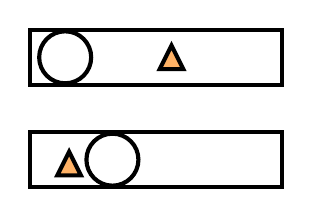
\begin{tikzpicture}
\draw[line width=1.5pt] (-1.6,0.55) rectangle (1.6,1.25);
\draw[line width=1.5pt] (-1.15,0.9) circle (0.13in);
\draw[fill=orange!60, line width=1.5pt] (0.05,0.75) -- (0.2,1.05) -- (0.35,0.75) -- cycle;
\draw[line width=1.5pt] (-1.6,-0.75) rectangle (1.6,-0.05);
\draw[fill=orange!60, line width=1.5pt] (-1.25,-0.6) -- (-1.1,-0.3) -- (-0.95,-0.6) -- cycle;
\draw[line width=1.5pt] (-0.55,-0.4) circle (0.13in);
\end{tikzpicture}
\vspace{0.2in}
{\large Rule: keep the order.}
\vspace{0.15in}\\
{\Huge Not equal.}
\end{center}
\pagenum{12}

\sprollpage
\begin{center}
\vspace*{0.7in}
\artnote{no new image; a calm closing scene, the four shapes from earlier, sitting unsorted, at rest}

\begin{tikzpicture}
\filldraw[fill=black] (-1.8,0) circle (0.13in);
\draw[line width=2pt] (-1.0,-0.13) rectangle (-0.6,0.13);
\draw[fill=orange!60] (0.3,-0.16) -- (0.5,0.16) -- (0.7,-0.16) -- cycle;
\draw[fill=orange!60] (1.5,0) circle (0.13in);
\end{tikzpicture}
\vspace{0.3in}
\bigline{``Are these equal'' is really asking:}\vspace{0.1in}
{\Large ``equal under which rule?''}
\end{center}
\pagenum{13}

\sprollpage
\begin{center}
\vspace*{0.5in}
\artnote{a small pile of connected pieces (a Bind structure) sitting beside a single whole shape, as if comparing a group of parts to something larger}

\begin{tikzpicture}
\filldraw[fill=black] (-1.5,0) circle (0.1in);
\filldraw[fill=black] (-1.2,0) circle (0.1in);
\draw[line width=1.5pt] (-1.38,0) -- (-1.32,0);
\draw[line width=1.5pt] (0.3,-0.3) rectangle (1.1,0.3);
\end{tikzpicture}
\vspace{0.3in}
\bigline{But what about a group made of many pieces?}\vspace{0.1in}
{\Large Can it be equal to the whole it became?}
\vspace{0.3in}\\
{\small \textit{--- turn the page for Sproll 09: Parts With a Past ---}}
\end{center}
\pagenum{14}

\sprollpage
\vspace*{0.3in}
{\large \textbf{A Note for Grown-Ups}}
\vspace{0.2in}

\normalsize
This book makes explicit what Sprolls 00 and 07 were building toward: equality is always relative to a rule, discovered by checking both sides against that rule, never assumed from appearance. The same objects can be equal under one rule and unequal under another, and neither judgment is more correct; each answers a different question.

\vspace{0.15in}
The four-shape sorting exercises are deliberately simple, but the underlying idea, that ``equal'' requires a stated basis for comparison, is exactly the idea used later in this curriculum wherever two constructed histories need to be compared. A child who has internalized ``equal under which rule'' here will not be surprised later by more demanding versions of the same question.

\vspace{0.3in}
{\small Sproll 09: Parts With a Past continues directly from this book's final page.}
\pagenum{15}

\end{document}
